\documentclass{article}
\usepackage[utf8]{inputenc}
\usepackage{graphicx}
\usepackage{mathtools} 
\usepackage{textcomp}
\usepackage{titling}
\usepackage{subfig}
\usepackage{amsmath}
\usepackage[parfill]{parskip}
\usepackage{xcolor}
\definecolor{LightGray}{gray}{0.9}
\usepackage{titlesec}
\setcounter{secnumdepth}{4}
\usepackage[a4paper,left=1cm,right=1cm,top=1cm,bottom=1.5cm,]{geometry}
\usepackage{eqparbox}
\usepackage{enumitem}

\title{\vspace{-2cm} DRAM Analysis}
\date{\vspace{-5ex}}

\begin{document}
\maketitle

\section{DRAM operation}
\begin{minipage}[c]{0.5\textwidth}
    \vspace{0pt}
    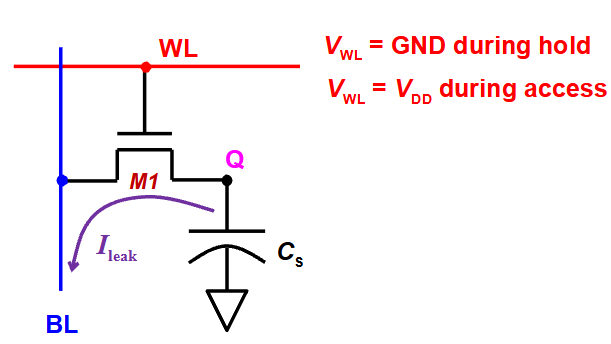
\includegraphics[width=9cm, scale=1]{dramOverview.PNG}
    \captionof{figure}{DRAM Bitcell}
\end{minipage}%
\begin{minipage}[c]{0.5\textwidth}
    Operation of DRAM is as follows \dots \newline

    \begin{itemize}
        \item Bitcell is \textit{accessed} to read or write data into the bitcell
            \begin{itemize}
                \item Electrically connect BL to \textit{storage node} Q
            \end{itemize}
        \item Otherwise, bitcell is in \textit{hold} mode and retains stored data
            \begin{itemize}
                \item Affected by leakage current $I_{leak}$
                \item Larger $C_{s}$ allows for more charge to be stored (and higher data retention time before refresh is required)
            \end{itemize}
    \end{itemize}
\end{minipage}

\subsection{DRAM Write}
\begin{minipage}[t]{0.5\textwidth}
    \centering
    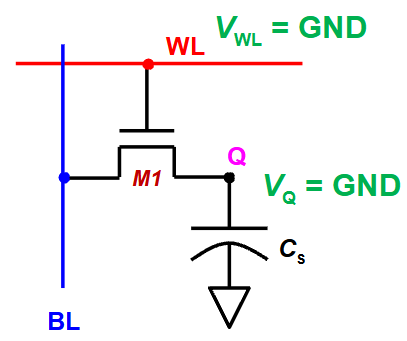
\includegraphics[width=5cm, scale=1]{dramWrite_1.PNG}
    \captionsetup{justification=centering}
    \captionof{figure}{Initial state\\
                        WL is off, capacitor charge is zero}
\end{minipage}%
\begin{minipage}[t]{0.5\textwidth}
    \centering
    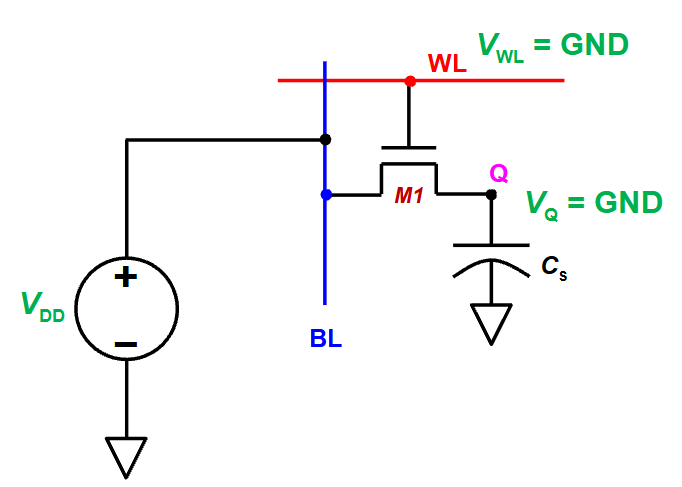
\includegraphics[width=6cm, scale=1]{dramWrite_2.PNG}
    \captionsetup{justification=centering}
    \captionof{figure}{Suppose we want to write \textbf{1}\\
                        Precharge BL to $V_{DD}$}
\end{minipage}%

\begin{minipage}[t]{0.5\textwidth}
    \centering
    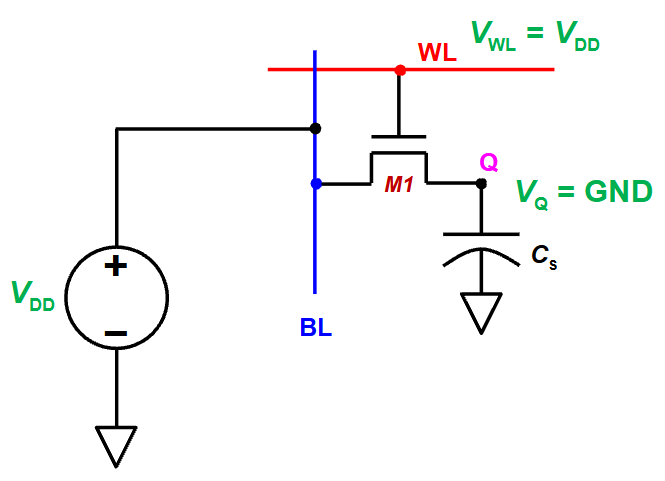
\includegraphics[width=6cm, scale=1]{dramWrite_3.PNG}
    \captionsetup{justification=centering}
    \captionof{figure}{Turn on WL}
\end{minipage}%
\begin{minipage}[t]{0.5\textwidth}
    \centering
    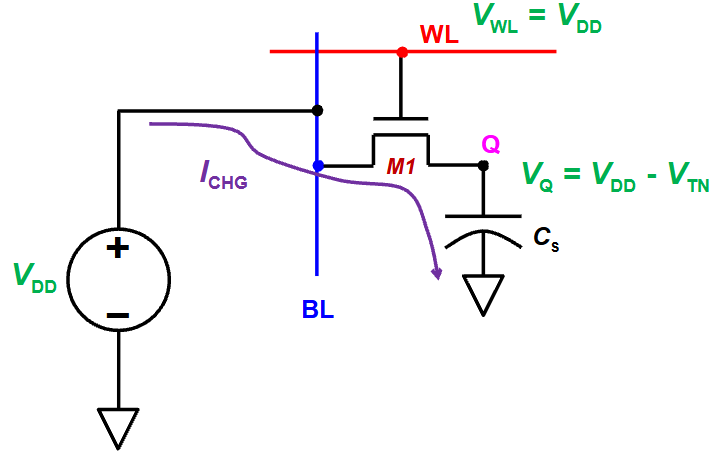
\includegraphics[width=6cm, scale=1]{dramWrite_4.PNG}
    \captionsetup{justification=centering}
    \captionof{figure}{Current flows into $C_{s}$\\
                        NMOS passes weak 1, therefore $V_{Q}$ goes up to $V_{DD} - V_{TH}$}
\end{minipage}%

\begin{figure}[htp]
    \centering
    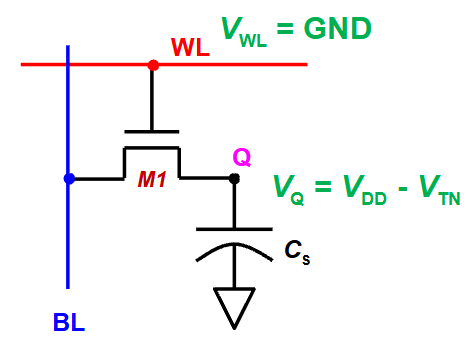
\includegraphics[width=6cm, scale=1]{dramWrite_5.PNG}
    \caption{Data successfully written into bitcell\\
                WL can be turned off, voltage at BL can be removed}
\end{figure}

\newpage
\subsection{DRAM Read}

\begin{minipage}[t]{0.5\textwidth}
    \centering
    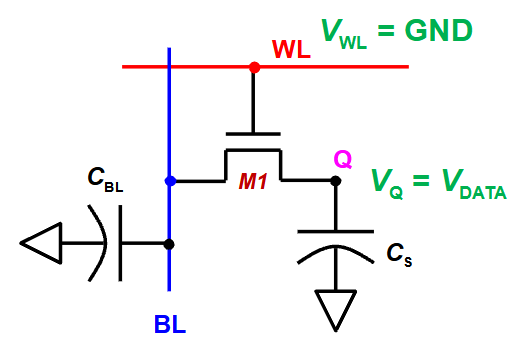
\includegraphics[width=6cm, scale=1]{dramRead_1.PNG}
    \captionsetup{justification=centering}
    \captionof{figure}{We want to read $V_{DATA}$ stored on $V_{Q}$\\
                        Notice that there is parasitic $C_{BL}$ on BL}
\end{minipage}%
\begin{minipage}[t]{0.5\textwidth}
    \centering
    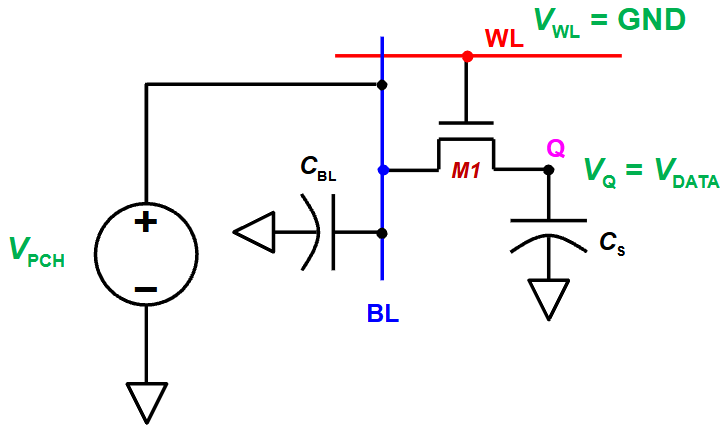
\includegraphics[width=6cm, scale=1]{dramRead_2.PNG}
    \captionsetup{justification=centering}
    \captionof{figure}{Precharge BL to $V_{PCH}$\\
                        Note that $V_{PCH}$ may be lower than $V_{DD}$}
\end{minipage}%

\begin{minipage}[t]{0.5\textwidth}
    \centering
    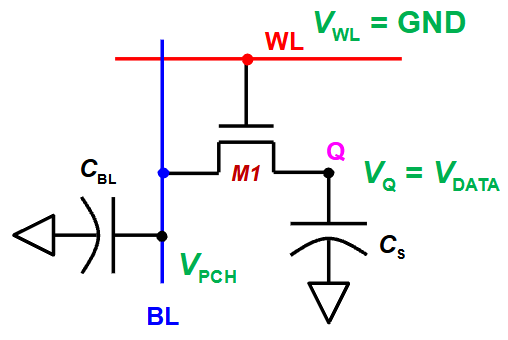
\includegraphics[width=6cm, scale=1]{dramRead_3.PNG}
    \captionsetup{justification=centering}
    \captionof{figure}{$C_{BL}$ now holds onto $V_{PCH}$\\
                        ie. high impedance node}
\end{minipage}%
\begin{minipage}[t]{0.5\textwidth}
    \centering
    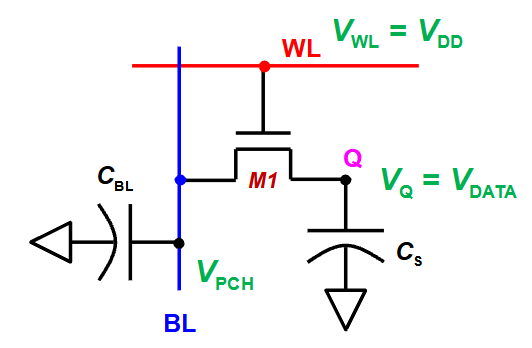
\includegraphics[width=6cm, scale=1]{dramRead_4.PNG}
    \captionsetup{justification=centering}
    \captionof{figure}{Turn on the WL, short-circuiting $C_{S}$ with $C_{BL}$\\
                        \textit{Charge-sharing} occurs}
\end{minipage}%

\subsubsection{Charge Sharing}
\begin{minipage}[c]{0.5\textwidth}
    \vspace{0pt}
    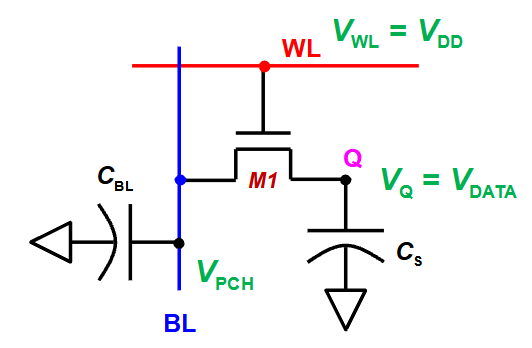
\includegraphics[width=9cm, scale=1]{dramRead_4.PNG}
    \captionof{figure}{Charge Sharing}
\end{minipage}%
\begin{minipage}[c]{0.5\textwidth}
    \begin{itemize}
        \item $Q_{S} = C_{S}V_{DATA}$
        \item $Q_{BL} = C_{BL}V_{PCH}$
        \item $Q_{TOTAL} = Q_{BL} + Q_{S}$
    \end{itemize}

    \vspace{0.5cm}
    When M1 turns on \dots
    \begin{itemize}
        \item $\Delta V_{BL} = \frac{Q_{TOTAL}}{C_{BL} + C_{S}} - V_{PCH}$
        \item $\Delta V_{Q} = \frac{Q_{TOTAL}}{C_{BL} + C_{S}} - V_{DATA}$
    \end{itemize}
\end{minipage}

\vspace{1cm}
\begin{minipage}[c]{0.5\textwidth}
    \vspace{0pt}
    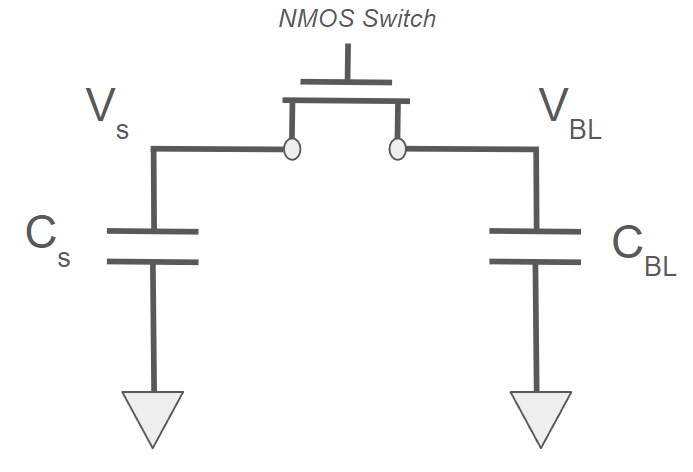
\includegraphics[width=9cm, scale=1]{dramRead_alternative.PNG}
    \captionof{figure}{Charge Sharing (Alternative view)}
\end{minipage}%
\begin{minipage}[c]{0.5\textwidth}
    $\underbrace{C_{S}V_{S} + C_{BL} \frac{V_{DD}}{2}}_{\text{Initial charge; NMOS open}}$ 
    =
    $\underbrace{(C_{S} + C_{BL}) V_{common}}_{\text{After charge sharing; NMOS closed}}$ 

    \vspace{0.5cm}
    \begin{itemize}
        \item If store \textbf{1}, then $V_{S} = V_{DD}$
        \item Assume that $V_{BL}$ is precharged to $\frac{V_{DD}}{2}$
    \end{itemize}

    \vspace{0.5cm}
    We can rearrange the above equation to get \dots \\
    \vspace{0.25cm}
    $\Delta V_{BL} = V_{common} - V_{BL} = \frac{C_{S}}{C_{S} + C_{BL}} \cdot \frac{V_{DD}}{2}$
    \vspace{0.25cm} \\
    From this, we can see that we want $C_{S} >>> C_{BL}$

\end{minipage}

\subsubsection{Sense Amplifier and Writeback}
\begin{minipage}[c]{0.5\textwidth}
    \vspace{0pt}
    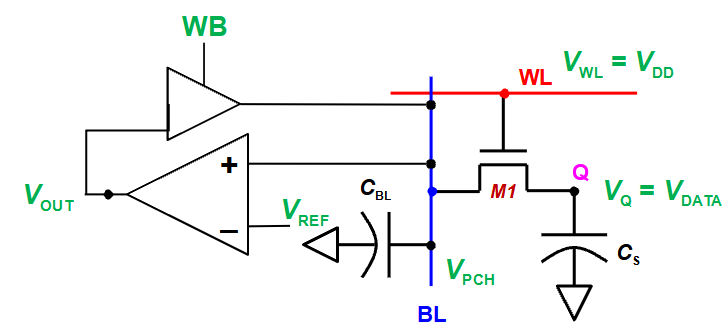
\includegraphics[width=9cm, scale=1]{dramRead_chargeSensing.PNG}
    \captionof{figure}{Op-amp with writeback}
\end{minipage}%
\begin{minipage}[c]{0.5\textwidth}
    \begin{itemize}
        \item $V_{REF}$ must be tuned correctly
        \item WB ensures that we rectify our destructive read
    \end{itemize}
\end{minipage}







\end{document}